\documentclass[11pt,a4paper]{report}
\usepackage[textwidth=37em,vmargin=30mm]{geometry}
\usepackage{calc,xunicode,amsmath,amssymb,paralist,enumitem,tabu,booktabs,datetime2,xeCJK,xeCJKfntef,listings}
\usepackage{tocloft,fancyhdr,tcolorbox,xcolor,graphicx,eso-pic,xltxtra,xelatexemoji}

\newcommand{\envyear}[0]{2025}
\newcommand{\envdatestr}[0]{2025-07-28}
\newcommand{\envfinaldir}[0]{webdb/2025/20250728/final}

\usepackage[hidelinks]{hyperref}
\hypersetup{
    colorlinks=false,
    pdfpagemode=FullScreen,
    pdftitle={Web Digest - \envdatestr}
}

\setlength{\cftbeforechapskip}{10pt}
\renewcommand{\cftchapfont}{\rmfamily\bfseries\large\raggedright}
\setlength{\cftbeforesecskip}{2pt}
\renewcommand{\cftsecfont}{\sffamily\small\raggedright}

\setdefaultleftmargin{2em}{2em}{1em}{1em}{1em}{1em}

\usepackage{xeCJK,xeCJKfntef}
\xeCJKsetup{PunctStyle=plain,RubberPunctSkip=false,CJKglue=\strut\hskip 0pt plus 0.1em minus 0.05em,CJKecglue=\strut\hskip 0.22em plus 0.2em}
\XeTeXlinebreaklocale "zh"
\XeTeXlinebreakskip = 0pt


\setmainfont{Brygada 1918}
\setromanfont{Brygada 1918}
\setsansfont{IBM Plex Sans}
\setmonofont{JetBrains Mono NL}
\setCJKmainfont{Noto Serif CJK SC}
\setCJKromanfont{Noto Serif CJK SC}
\setCJKsansfont{Noto Sans CJK SC}
\setCJKmonofont{Noto Sans CJK SC}

\setlength{\parindent}{0pt}
\setlength{\parskip}{8pt}
\linespread{1.15}

\lstset{
	basicstyle=\ttfamily\footnotesize,
	numbersep=5pt,
	backgroundcolor=\color{black!5},
	showspaces=false,
	showstringspaces=false,
	showtabs=false,
	tabsize=2,
	captionpos=b,
	breaklines=true,
	breakatwhitespace=true,
	breakautoindent=true,
	linewidth=\textwidth
}






\newcommand{\coverpic}[2]{
    % argv: itemurl, authorname
    Cover photo by #2~~(\href{#1}{#1})
}
\newcommand{\makeheader}[0]{
    \begin{titlepage}
        % \newgeometry{hmargin=15mm,tmargin=21mm,bmargin=12mm}
        \begin{center}
            
            \rmfamily\scshape
            \fontspec{BaskervilleF}
            \fontspec{Old Standard}
            \fontsize{59pt}{70pt}\selectfont
            WEB\hfill DIGEST
            
            \vfill
            % \vskip 30pt
            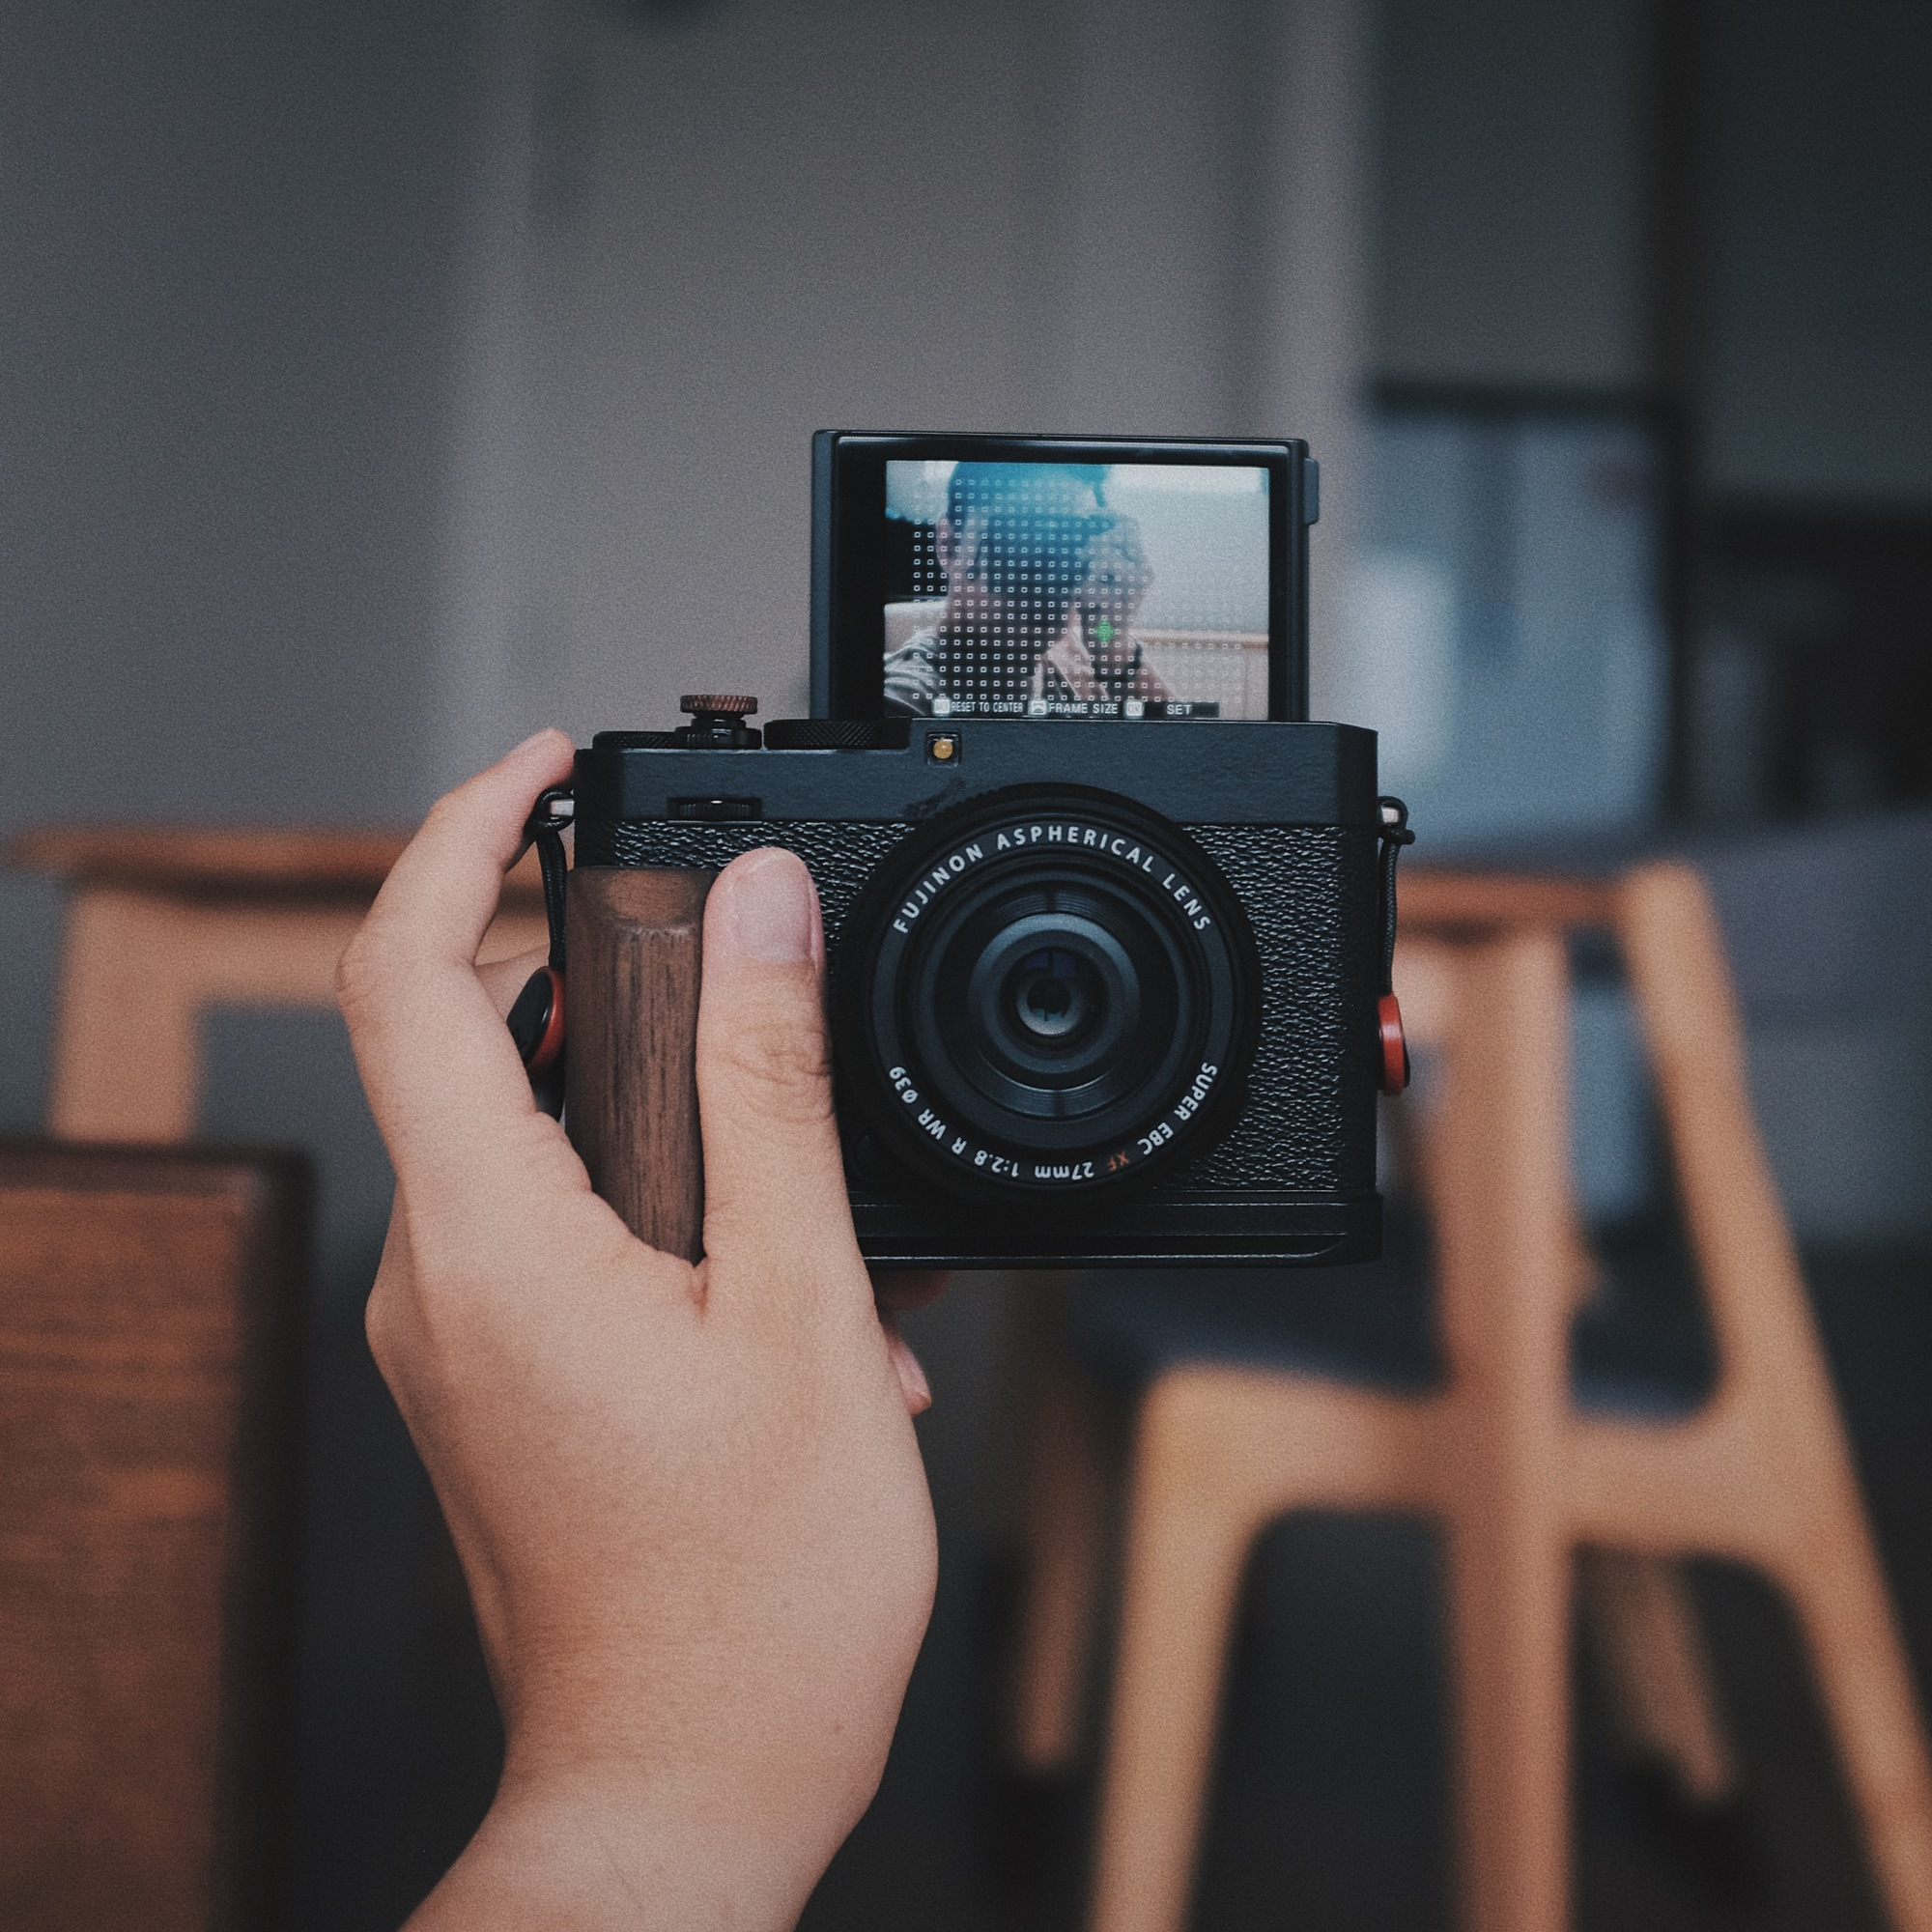
\includegraphics[width=\linewidth]{\envfinaldir/coverpic-prod.jpg}\par
            % \vskip 30pt
            \vfill

            \normalsize\rmfamily\scshape
            \copyright{} The Web Digest Project \hfill\large \envdatestr
        \end{center}
    \end{titlepage}
    % \restoregeometry
}
\newcommand{\simplehref}[1]{%
    \textcolor{blue!80!green}{\href{#1}{#1}}%
}
\renewcommand{\contentsname}{\center\Huge\sffamily\bfseries Contents\par\vskip 20pt}
\newcounter{ipartcounter}
\setcounter{ipartcounter}{0}
\newcommand{\ipart}[1]{
    % \vskip 20pt
    \clearpage
    \stepcounter{ipartcounter}
    \phantomsection
    \addcontentsline{toc}{chapter}{#1}
    % \begin{center}
    %     \Huge
    %     \sffamily\bfseries
    %     #1
    % \end{center}
    % \vskip 20pt plus 7pt
}
\newcounter{ichaptercounter}
\setcounter{ichaptercounter}{0}
\newcommand{\ichapter}[1]{
    % \vskip 20pt
    \clearpage
    \stepcounter{ichaptercounter}
    \phantomsection
    \addcontentsline{toc}{section}{\numberline{\arabic{ichaptercounter}}#1}
    \begin{center}
        \Huge
        \sffamily\bfseries
        #1
    \end{center}
    \vskip 20pt plus 7pt
}
\newcommand{\entrytitlefont}[1]{\subsection*{\raggedright\Large\sffamily\bfseries#1}}
\newcommand{\entryitemGeneric}[2]{
    % argv: title, url
    \parbox{\linewidth}{
        \entrytitlefont{#1}\par\vskip 5pt
        \footnotesize\ttfamily\mdseries
        \simplehref{#2}
    }\vskip 11pt plus 11pt minus 1pt
}
\newcommand{\entryitemGithub}[3]{
    % argv: title, url, desc
    \parbox{\linewidth}{
        \entrytitlefont{#1}\par\vskip 5pt
        \footnotesize\ttfamily\mdseries
        \simplehref{#2}\par\vskip 5pt
        \small\rmfamily\mdseries#3
    }\vskip 11pt plus 11pt minus 1pt
}
\newcommand{\entryitemAp}[3]{
    % argv: title, url, desc
    \parbox{\linewidth}{
        \entrytitlefont{#1}\par\vskip 5pt
        \footnotesize\ttfamily\mdseries
        \simplehref{#2}\par\vskip 5pt
        \small\rmfamily\mdseries#3
    }\vskip 11pt plus 11pt minus 1pt
}
\newcommand{\entryitemHackernews}[3]{
    % argv: title, hnurl, rawurl
    % \parbox{\linewidth}{
    %     \entrytitlefont{#1}\par\vskip 5pt
    %     \footnotesize\ttfamily\mdseries
    %     \simplehref{#3}\par
    %     \textcolor{black!50}{\href{#2}{#2}}
    % }\vskip 11pt plus 11pt minus 1pt
    \begin{minipage}{\linewidth}
            \entrytitlefont{#1}\par\vskip 5pt
            \footnotesize\ttfamily\mdseries
            \simplehref{#3}\par
            \textcolor{black!50}{\href{#2}{#2}}
    \end{minipage}\par\vskip 11pt plus 11pt minus 1pt
}







\begin{document}

\makeheader

\tableofcontents\clearpage




\ipart{Developers}
\ichapter{Hacker News}
\entryitemTwoLinks{EU age verification app to ban any Android system not licensed by Google}{https://news.ycombinator.com/item?id=44705240}{https://www.reddit.com/r/degoogle/s/YxmPgFes8a}

\entryitemTwoLinks{Making Postgres slower}{https://news.ycombinator.com/item?id=44704736}{https://byteofdev.com/posts/making-postgres-slow/}

\entryitemTwoLinks{Performance and Telemetry Analysis of Trae IDE, ByteDance's VSCode Fork}{https://news.ycombinator.com/item?id=44703164}{https://github.com/segmentationf4u1t/trae\_telemetry\_research}

\entryitemTwoLinks{Allianz Life says 'majority' of customers' personal data stolen in cyberattack}{https://news.ycombinator.com/item?id=44703079}{https://techcrunch.com/2025/07/26/allianz-life-says-majority-of-customers-personal-data-stolen-in-cyberattack/}

\entryitemTwoLinks{Show HN: Windows 7 GUI for the web}{https://news.ycombinator.com/item?id=44702894}{https://khang-nd.github.io/7.css/}

\entryitemTwoLinks{Ask HN: What are you working on? (July 2025)}{https://news.ycombinator.com/item?id=44702833}{https://news.ycombinator.com/item?id=44702833}

\entryitemTwoLinks{Tom Lehrer has died}{https://news.ycombinator.com/item?id=44702782}{https://www.nytimes.com/2025/07/27/arts/music/tom-lehrer-dead.html}

\entryitemTwoLinks{Claude Code is a slot machine}{https://news.ycombinator.com/item?id=44702046}{https://rgoldfinger.com/blog/2025-07-26-claude-code-is-a-slot-machine/}

\entryitemTwoLinks{The many JavaScript runtimes of the last decade}{https://news.ycombinator.com/item?id=44701574}{https://buttondown.com/whatever\_jamie/archive/the-many-many-many-javascript-runtimes-of-the-last-decade/}

\entryitemTwoLinks{Dumb Pipe}{https://news.ycombinator.com/item?id=44701555}{https://www.dumbpipe.dev/}

\entryitemTwoLinks{Beetroot juice lowers blood pressure by changing oral microbiome: study}{https://news.ycombinator.com/item?id=44700923}{https://news.exeter.ac.uk/faculty-of-health-and-life-sciences/beetroot-juice-lowers-blood-pressure-in-older-people-by-changing-oral-microbiome/}

\entryitemTwoLinks{Hierarchical Reasoning Model}{https://news.ycombinator.com/item?id=44699452}{https://arxiv.org/abs/2506.21734}

\entryitemTwoLinks{When we get Komooted}{https://news.ycombinator.com/item?id=44699421}{https://bikepacking.com/plog/when-we-get-komooted/}

\entryitemTwoLinks{Linux on Snapdragon X Elite: Linaro and Tuxedo Pave the Way for ARM64 Laptops}{https://news.ycombinator.com/item?id=44699393}{https://www.linaro.org/blog/linux-on-snapdragon-x-elite/}

\entryitemTwoLinks{4k NASA employees opt to leave agency through deferred resignation program}{https://news.ycombinator.com/item?id=44699052}{https://www.kcrw.com/news/shows/npr/npr-story/nx-s1-5481304}

\entryitemTwoLinks{Chemical process produces critical battery metals with no waste}{https://news.ycombinator.com/item?id=44698928}{https://spectrum.ieee.org/nmc-battery-aspiring-materials}

\entryitemTwoLinks{The future is not self-hosted, but self-sovereign}{https://news.ycombinator.com/item?id=44698899}{https://www.robertmao.com/blog/en/the-future-is-not-self-hosted-but-self-sovereign}

\entryitemTwoLinks{Fast and cheap bulk storage: using LVM to cache HDDs on SSDs}{https://news.ycombinator.com/item?id=44698754}{https://quantum5.ca/2025/05/11/fast-cheap-bulk-storage-using-lvm-to-cache-hdds-on-ssds/}

\entryitemTwoLinks{Smallest particulate matter air quality sensor for ultra-compact IoT devices}{https://news.ycombinator.com/item?id=44698733}{https://www.bosch-sensortec.com/news/worlds-smallest-particulate-matter-sensor-bmv080.html}

\entryitemTwoLinks{Janet: Lightweight, Expressive, Modern Lisp}{https://news.ycombinator.com/item?id=44698185}{https://janet-lang.org}


\ipart{Developers~~~~(zh-Hans)}
\ichapter{Solidot}
\entryitemGeneric{\hskip 0pt{}今天的环法自行车选手已经超越了当年的阿姆斯特朗}{https://www.solidot.org/story?sid=81900}

\entryitemGeneric{\hskip 0pt{}受争议的砷基生命论文在发表 15 年后撤下}{https://www.solidot.org/story?sid=81899}

\entryitemGeneric{\hskip 0pt{}Pebble 创始人拿回了原商标}{https://www.solidot.org/story?sid=81898}

\entryitemGeneric{\hskip 0pt{}地球在向外星人广播其位置}{https://www.solidot.org/story?sid=81897}

\entryitemGeneric{\hskip 0pt{}DNSSEC 普及率仅为 34\%}{https://www.solidot.org/story?sid=81896}

\entryitemGeneric{\hskip 0pt{}Google 街景车拍摄到阿根廷男子的裸体被判赔偿 1.25 万美元}{https://www.solidot.org/story?sid=81895}

\entryitemGeneric{\hskip 0pt{}Wayback 0.1 释出}{https://www.solidot.org/story?sid=81894}

\entryitemGeneric{\hskip 0pt{}AMD CEO 称台积电美国工厂制造的芯片贵 5\%-20\%}{https://www.solidot.org/story?sid=81893}

\entryitemGeneric{\hskip 0pt{}微软 CEO 轻淡的回应公司裁员之谜}{https://www.solidot.org/story?sid=81892}

\entryitemGeneric{\hskip 0pt{}Mistral AI 环境报告证实 AI 是一个饥渴的怪物}{https://www.solidot.org/story?sid=81891}

\entryitemGeneric{\hskip 0pt{}特朗普威胁关闭 TikTok }{https://www.solidot.org/story?sid=81890}

\entryitemGeneric{\hskip 0pt{}Debian 13.0 Trixie 的新变化}{https://www.solidot.org/story?sid=81889}

\entryitemGeneric{\hskip 0pt{}GPD 推出配备 Ryzen AI Max+ 395 的掌机}{https://www.solidot.org/story?sid=81888}

\entryitemGeneric{\hskip 0pt{}日本将允许用 iPS 细胞制造人类受精卵}{https://www.solidot.org/story?sid=81887}

\entryitemGeneric{\hskip 0pt{}英特尔今年将裁员 2.4 万人}{https://www.solidot.org/story?sid=81886}

\entryitemGeneric{\hskip 0pt{}2023 年的海洋热浪史无前例}{https://www.solidot.org/story?sid=81885}

\entryitemGeneric{\hskip 0pt{}CERN 演示反物质量子比特}{https://www.solidot.org/story?sid=81884}

\entryitemGeneric{\hskip 0pt{}国际法院认为健康环境是人权}{https://www.solidot.org/story?sid=81883}\ichapter{V2EX}
\entryitemGeneric{\hskip 0pt{}[RSS] follow 网页版不能用了吗}{https://www.v2ex.com/t/1148083}

\entryitemGeneric{\hskip 0pt{}[问与答] 车被施工飞漆,有点严重,该如何去维权}{https://www.v2ex.com/t/1148082}

\entryitemGeneric{\hskip 0pt{}[问与答] 第一次在官方通报里看到的单位是美刀}{https://www.v2ex.com/t/1148081}

\entryitemGeneric{\hskip 0pt{}[微信] 微信开发者工具?纯纯工业废料!}{https://www.v2ex.com/t/1148080}

\entryitemGeneric{\hskip 0pt{}[宽带症候群] 移动宽带通过 ZeroTier 组网时上传限速问题探究:非 UDP/端口限制,疑似特定策略触发}{https://www.v2ex.com/t/1148079}

\entryitemGeneric{\hskip 0pt{}[Solana] 学了一个新词,尘埃攻击}{https://www.v2ex.com/t/1148078}

\entryitemGeneric{\hskip 0pt{}[推广] 阿里云 ESA 现在有免费套餐了}{https://www.v2ex.com/t/1148077}

\entryitemGeneric{\hskip 0pt{}[输入法] 常逛小红书的输入法相关,结果今天被推送了一个``女性输入法''}{https://www.v2ex.com/t/1148076}

\entryitemGeneric{\hskip 0pt{}[Solana] 想问下大家对 V2EX 币的发展有什么见解?}{https://www.v2ex.com/t/1148075}

\entryitemGeneric{\hskip 0pt{}[搜索引擎优化] 分享一下可以用作外链的``个人主页''类的网站}{https://www.v2ex.com/t/1148074}

\entryitemGeneric{\hskip 0pt{}[VMware] vmware 蓝屏进不去 请问有哪些修理渠道?电脑城或者闲鱼?}{https://www.v2ex.com/t/1148073}

\entryitemGeneric{\hskip 0pt{}[问与答] macos 下有好用的 time-tracker 类的软件么?}{https://www.v2ex.com/t/1148072}

\entryitemGeneric{\hskip 0pt{}[Solana] v2ex 怎么买}{https://www.v2ex.com/t/1148070}

\entryitemGeneric{\hskip 0pt{}[健康] 脂溢性皮炎究竟该怎么治}{https://www.v2ex.com/t/1148068}

\entryitemGeneric{\hskip 0pt{}[问与答] 有哪些国家可以快速拿到签证并且好玩的地方}{https://www.v2ex.com/t/1148067}

\entryitemGeneric{\hskip 0pt{}[问与答] 汽车小白求推荐 10-15w 的纯电汽车}{https://www.v2ex.com/t/1148065}

\entryitemGeneric{\hskip 0pt{}[分享创造] SupermicroController-超微服务器 IPMI 控制脚本}{https://www.v2ex.com/t/1148064}

\entryitemGeneric{\hskip 0pt{}[大学] 免费 AI 论文生成器推荐: 6 款高效工具助你轻松写论文!}{https://www.v2ex.com/t/1148063}

\entryitemGeneric{\hskip 0pt{}[问与答] 病危患者的职工医保能否转灵活就业,如何操作?}{https://www.v2ex.com/t/1148062}

\entryitemGeneric{\hskip 0pt{}[Windows] 如何下载或编译得到 winget.exe?}{https://www.v2ex.com/t/1148061}

\entryitemGeneric{\hskip 0pt{}[问与答] 有懂车的 V 友么,老爸要换车,麻烦帮忙看看~}{https://www.v2ex.com/t/1148059}

\entryitemGeneric{\hskip 0pt{}[问与答] 平时搜索一般搜什么关键词(那方面}{https://www.v2ex.com/t/1148058}

\entryitemGeneric{\hskip 0pt{}[问与答] 分享自己觉得有用的 mcp?}{https://www.v2ex.com/t/1148057}

\entryitemGeneric{\hskip 0pt{}[推广] 项目分享: ElasticView 开发辅助工具管理平台}{https://www.v2ex.com/t/1148056}

\entryitemGeneric{\hskip 0pt{}[问与答] 有个朋友变得不爱和人交流这真的不好吗?}{https://www.v2ex.com/t/1148055}

\entryitemGeneric{\hskip 0pt{}[问与答] 疑似微博被盗号?}{https://www.v2ex.com/t/1148054}

\entryitemGeneric{\hskip 0pt{}[Android] 求推荐个二手八九百的安卓备机}{https://www.v2ex.com/t/1148053}

\entryitemGeneric{\hskip 0pt{}[分享创造] 从构想走向现实:一个 AI Agent 开发者的实践手记}{https://www.v2ex.com/t/1148052}

\entryitemGeneric{\hskip 0pt{}[程序员] 拖延症晚期如何解决}{https://www.v2ex.com/t/1148051}

\entryitemGeneric{\hskip 0pt{}[Apple] 请教开通 AirPods 助听器功能}{https://www.v2ex.com/t/1148050}

\entryitemGeneric{\hskip 0pt{}[宽带症候群] 最近发现扬州电信 ip 段被很多 waf 直接默认屏蔽了}{https://www.v2ex.com/t/1148049}

\entryitemGeneric{\hskip 0pt{}[程序员] 发现一个最简单的免费部署纯静态网站的方法: surge.sh}{https://www.v2ex.com/t/1148048}

\entryitemGeneric{\hskip 0pt{}[问与答] 为什么群晖 transmission 上行被限速 500kb、webdav 看电影 200kb、但是家庭宽带测速就是正常 50Mbps 呢?}{https://www.v2ex.com/t/1148046}

\entryitemGeneric{\hskip 0pt{}[Android] 分享一个小米不用跑路解锁 BL 的方案}{https://www.v2ex.com/t/1148044}

\entryitemGeneric{\hskip 0pt{}[分享发现] Debian 服务器通过 rclone 挂载缤纷云(或其他 s3 兼容云存储),适用宝塔备份任务}{https://www.v2ex.com/t/1148043}

\entryitemGeneric{\hskip 0pt{}[职场话题] 今天星期天,想问下有多少朋友的生活是 996}{https://www.v2ex.com/t/1148041}

\entryitemGeneric{\hskip 0pt{}[分享创造] 又感受到写博客的意义了}{https://www.v2ex.com/t/1148040}

\entryitemGeneric{\hskip 0pt{}[Apple] mac M2 迁移到 M4 国补 7k 不到拿下 24+512}{https://www.v2ex.com/t/1148039}

\entryitemGeneric{\hskip 0pt{}[分享发现] 眼看 v 站从技术社区变成情感论坛又变成了炒币论坛}{https://www.v2ex.com/t/1148037}

\entryitemGeneric{\hskip 0pt{}[职场话题] 领导跑路了,现在去还是留}{https://www.v2ex.com/t/1148035}

\entryitemGeneric{\hskip 0pt{}[问与答] 为什么王者荣耀的生命周期这么长?}{https://www.v2ex.com/t/1148034}

\entryitemGeneric{\hskip 0pt{}[职场话题] 前公司拖欠工资两年多了竟然还有人自己交社保在上班}{https://www.v2ex.com/t/1148033}

\entryitemGeneric{\hskip 0pt{}[问与答] 转行申论老师。已经有不少学生上岸了。各位有什么想提问的吗?}{https://www.v2ex.com/t/1148032}

\entryitemGeneric{\hskip 0pt{}[投资] 工程师如何更好投资}{https://www.v2ex.com/t/1148031}

\entryitemGeneric{\hskip 0pt{}[Mac mini] [求助] Macmini M4 拔掉扩展坞 wifi 立刻没网}{https://www.v2ex.com/t/1148030}

\entryitemGeneric{\hskip 0pt{}[酷工作] 有个埃及的工作岗位,有需要的可以和我联系}{https://www.v2ex.com/t/1148029}

\entryitemGeneric{\hskip 0pt{}[程序员] 为什么永远有人在一谈到计算机/编程就要说自学呢?为什么?}{https://www.v2ex.com/t/1148028}

\entryitemGeneric{\hskip 0pt{}[Android] 三星 One UI 8 移除 Bootloader 解锁功能}{https://www.v2ex.com/t/1148026}

\entryitemGeneric{\hskip 0pt{}[macOS] 如何通过 smb 访问连接在 mac 上的外接硬盘?}{https://www.v2ex.com/t/1148025}

\entryitemGeneric{\hskip 0pt{}[Windows] Win11 用 PowerToys 的键盘管理器设置热键有时有效有时不生效}{https://www.v2ex.com/t/1148024}


\ipart{Generic News}







\clearpage
\leavevmode\vfill
\footnotesize

Copyright \copyright{} 2023-2025 Neruthes and other contributors.

This document is published with CC BY-NC-ND 4.0 license.

The entries listed in this newsletter may be copyrighted by their respective creators.

This newsletter is generated by the Web Digest project.

The newsletters are also delivered via Telegram channel \CJKunderline{\href{https://t.me/webdigestchannel}{https://t.me/webdigestchannel}}.\\
RSS feed is available at \CJKunderline{\href{https://webdigest.pages.dev/rss.xml}{https://webdigest.pages.dev/rss.xml}}.

This newsletter is available in PDF at
\CJKunderline{\href{https://webdigest.pages.dev/}{https://webdigest.pages.dev/}}.

The source code being used to generate this newsletter is available at\\
\CJKunderline{\href{https://github.com/neruthes/webdigest}{https://github.com/neruthes/webdigest}}.

This newsletter is also available in
\CJKunderline{\href{http://webdigest.pages.dev/readhtml/\envyear/WebDigest-20250728.html}{HTML}} and
\CJKunderline{\href{https://github.com/neruthes/webdigest/blob/master/markdown/\envyear/WebDigest-20250728.md}{Markdown}}.


\coverpic{https://unsplash.com/photos/large-green-leaves-stand-tall-in-the-sunlight-xhkUiqHUWRI}{Vidit Goswami}


\end{document}
